% !TEX TS-program = pdflatex
% !TEX encoding = UTF-8 Unicode

\documentclass[11pt]{article} % use larger type; default would be 10pt
\usepackage[utf8]{inputenc} % set input encoding (not needed with XeLaTeX)

\usepackage{hyperref}

\usepackage{geometry} % to change the page dimensions
\geometry{a4paper} % or letterpaper (US) or a5paper or....
% \geometry{margin=2in} % for example, change the margins to 2 inches all round
% \geometry{landscape} % set up the page for landscape
%   read geometry.pdf for detailed page layout information

\usepackage{graphicx}

% \usepackage[parfill]{parskip} % Activate to begin paragraphs with an empty line rather than an indent

\usepackage{booktabs} % for much better looking tables
\usepackage{array} % for better arrays (eg matrices) in maths
\usepackage{paralist} % very flexible & customisable lists (eg. enumerate/itemize, etc.)
\usepackage{verbatim} % adds environment for commenting out blocks of text & for better verbatim
\usepackage{subfig} % make it possible to include more than one captioned figure/table in a single float

\usepackage{fancyhdr} % This should be set AFTER setting up the page geometry
\pagestyle{fancy} % options: empty , plain , fancy
\renewcommand{\headrulewidth}{0pt} % customise the layout...
\lhead{}\chead{}\rhead{}
\lfoot{}\cfoot{\thepage}\rfoot{}

\usepackage{sectsty}
\allsectionsfont{\sffamily\mdseries\upshape} % (See the fntguide.pdf for font help)
% (This matches ConTeXt defaults)

\usepackage[nottoc,notlof,notlot]{tocbibind} % Put the bibliography in the ToC
\usepackage[titles,subfigure]{tocloft} % Alter the style of the Table of Contents
\renewcommand{\cftsecfont}{\rmfamily\mdseries\upshape}
\renewcommand{\cftsecpagefont}{\rmfamily\mdseries\upshape} % No bold!

\setcounter{secnumdepth}{-1} 

\title{
\begin{figure}[htb]
\centering
\includegraphics[scale=0.5]{Four-color-deck.png}
\label{Logo}
\end{figure}
Shuffle-Spires
}
\author{Eric Nilsson}
\date{}
\begin{document}
\maketitle

\noindent
\textbf{Shuffle-Spires} is a smaller card-/dice-/board-game designed around four players, using only a standard deck of cards and a D10 (ten sided die). \\
All you need in order to play \textbf{Shuffle-Spires} is:
\begin{itemize}
\renewcommand{\labelitemi}{$\bullet$}
\item a set of playing cards
\item one of those dice* I mentioned earlier
\item this rule-set
\item ...and some friends
\end{itemize}
\textbf{Shuffle-Spires} may be played with two or four players.

\noindent
{\it*In the event of having lost your personal D10; cards from another deck numbered one through ten (Ace being nr. 1) may be used as an improvised randomization-device.} \\
{\it*If you do not own a D10; then congratulations - you seem to be the owner of something we nerds would refer to as ‘social lifestyle’. Please ditch this rule-set in the nearest bin and resume enjoying your life.}

\subsection{Legend of the Shuffling Spires of Thin}
Old tales tell of the mystic Kingdoms of Thin, all of which border in four equally divided parts of a circle - in the Realm of Thin-Things.
These kingdoms were ruled by four power-hungry Kings, each jealous of the next, their fair Queens, brave Jacks and top 10 Henchmen numbered - you guessed it - one through ten. \\
Even though the Kings’ respective wealth were great, they were not content with ruling only one of the Kingdoms of Thin. Each wanted to claim the entire Realm for their own. Since all Kingdoms were equally thin, this would require very precise plotting. \\
...and we all know that plotting means spying, and you cannot spell ‘spyglass’ without ‘spy’, and the only way to use a spyglass effectively is to use it from something very wide, lengthy or high. \\ 
\noindent
Since width is hard to come by in the Realm of Thin-Things, and ‘length’ is a more bothersome word, the Kings all plotted to construct high Spires, so they could spy far-away from their Kingdom - for the right moment when they could claim the Realm for themselves.

\noindent
The problem with spires, though, is that they’re immobile - and once you’ve placed a spire it may be hard to move it if one would wish to spy somewhere else. After all, to dominate the Realm of Thin-Things, one would have to spy on all four Kingdoms! \\

\noindent
Luckily, in the Lands of Thin, one may construct remarkably thin-things. So the Kings plotted to build four equally high and thin spires, all constructed in three very - even in the Realm of Thin-Things - thin sections. The low parts were assigned to the Jacks, who were the most suitable 'Thins' to guard and protect the towers, the middle bits were assigned to the Queens and the highest sections were given unto the Kings themselves.

\noindent
These sections were so amazingly thin that the wind would easily carry them anywhere across the Lands of Thin. This way; the Kings could spy on all of their neighbours in wait for the right moment to strike. \\

\noindent
When this opportunity had come (when the stars were right, if you will) it was decided that the Kingdoms’ ten best Henchmen were to launch an all-out assault targeted at the other Kingdoms. This would be the way to a unified Realm of Thin-Things, thought the Kings. \\
And so one day a mighty storm swept the Kingdoms of Thin and took even the least-thin Henchmen aloft. The Realm was veiled in powerful winds, the likes of which neither Kingdom had ever seen. In the midst of all this chaos, all four Kings decided to put their respective master plan to work and gaze from their high Spires as they conquered the Lands of Thin.

\noindent
But it came to pass that the Kings of Thin were also men of thin intellect, as it did not occur to them that their high Spires had also been swept from the lands and were being taken far away from their Kingdom. The High Spires of Thin were swept across the Realm, across the Kingdoms of Thin and shuffled so that neither King knew what Kingdom nor Spire he was in.
Yet neither side's Henchmen saw any difference. \\
\noindent
The Kings and their Shuffling Spires were about to be attacked by not only the other armies, but by their own. \\

\noindent Thus, the Legend of the Shuffling Spires of Thin was made. \\

\textbf{Shuffle-Spires} is based around the four Kings, and the Legendary Spires of Thin.

\subsection{Setting up the board}
Like most things in the Realm of Thin-Things, there is not much room for humour. Therefore, the joker has no place in either Kingdom. Remove all jokers from the deck.\\

\noindent
The \textbf{Shuffle-Spires} board is set up using the Kings, Queens and Jacks (of all suits) to represent the four Spires and their three sections. One could imagine the Spires stretching outward from the center. Shuffle the rest of the deck, containing cards one-through-ten (Ace being nr. 1) from all suits, and place it in the middle of the board.
The Spires thusly create three different zones on the board, which will represent progression of the attacking Henchmen.
Each player chooses a King (a suit, rather), and places him-/herself next to the currently inhabited Spire. Note that the player is not the owner of any specific Spire, but rather three parts that will change location during play. \\
If there are but two players, each player controls two Kings (suits) each. \\

\noindent
The King of Hearts starts off with the title \textit{'The Thin-Things-Thin'}, to signify him being the current Ruler of the Realm of Thin-Things. This title dictates when the Henchmen are moved further towards the center of the Spires. This title may be given unto someone else during play.

\begin{figure}[h!]
\centering
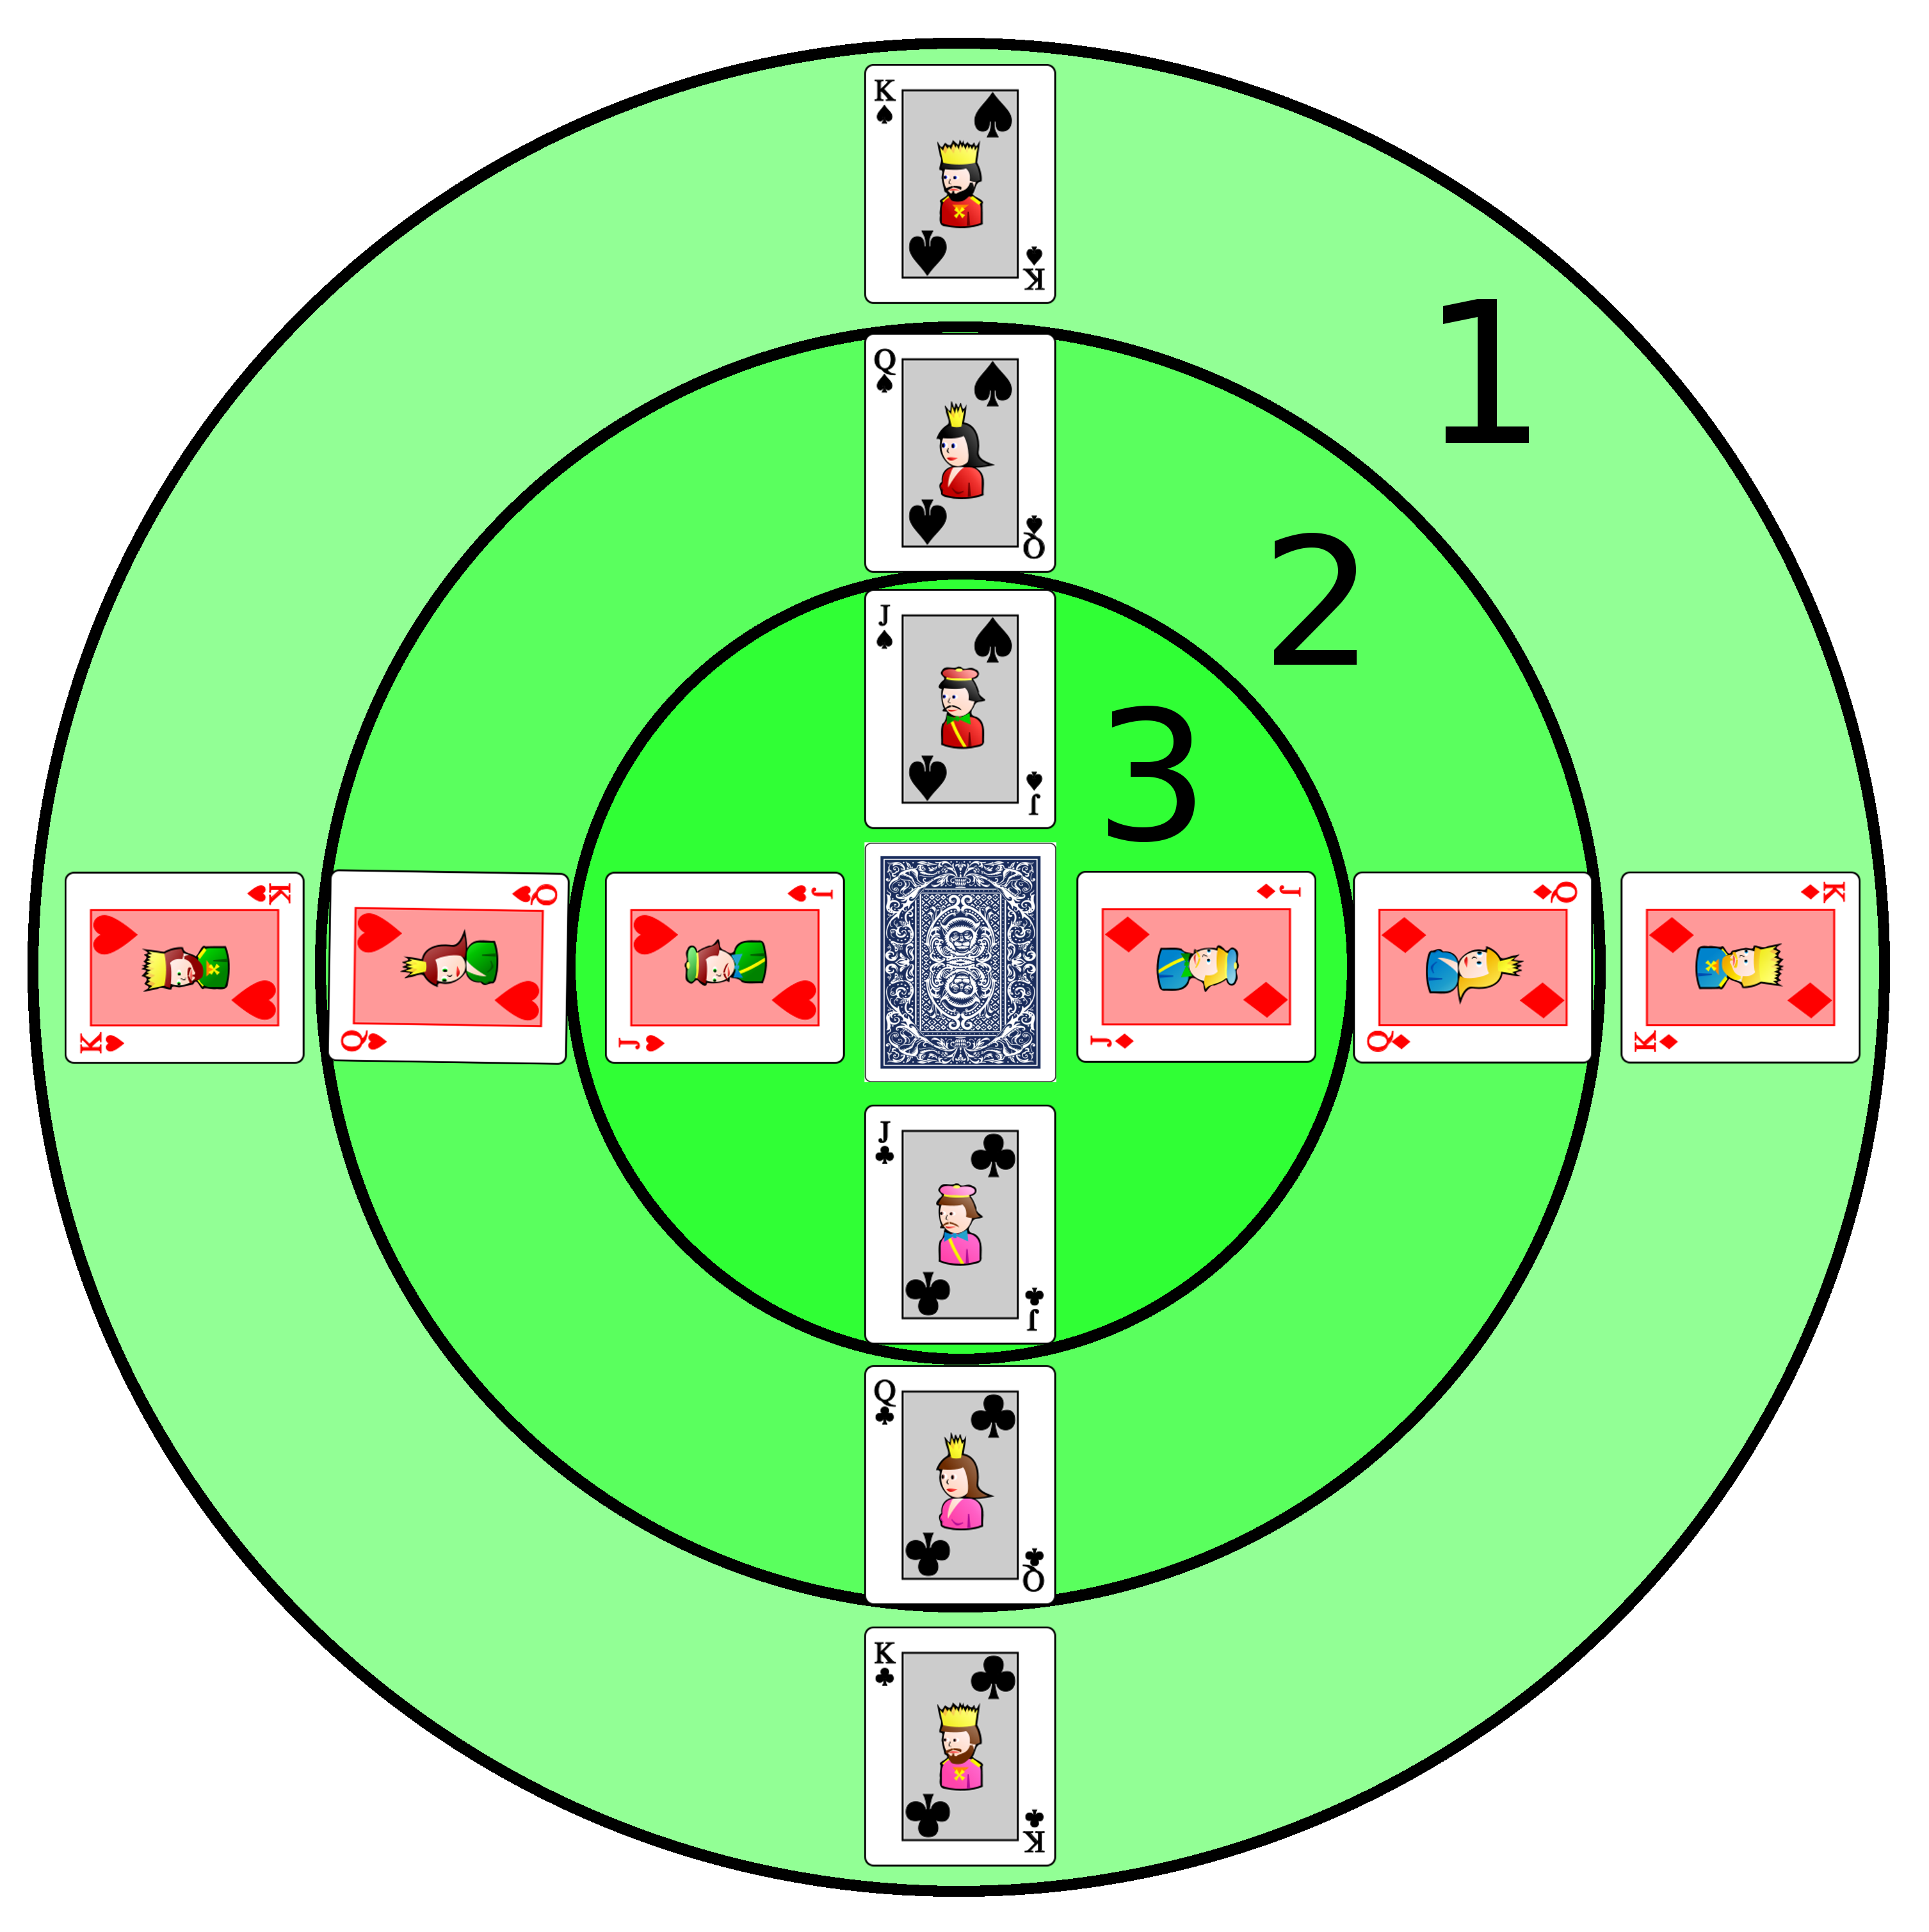
\includegraphics[scale=0.08]{starting.png}
\caption{Starting board and progression zones}
\label{starting}
\end{figure}

\subsection{Note}
Since the Spires may shuffle and swap during play, \textit{'X's Spire'} will signify the Spire Player X's King currently resides in.

\subsection{Playing \textbf{Shuffle-Spires}}
Shuffle-Spires is a turn-based game, wherein a turn has four independent steps in a strict order:
\begin{itemize}
\renewcommand{\labelitemi}{$\bullet$}
\item  Progression
\item Draw
\item Attack
\item Shuffle
\end{itemize}
Turn-progression is clockwize.

\subsubsection{Progression-phase}
If you’re the current \textit{Thin-Things-Thin}; move all attacking Henchmen one step forward. (\textit{Zone 1} to \textit{Zone 2} etc.) \\
When the previous owner of this title is slain; the title of \textit{Thin-Things-Thin} is simply given unto the next player. (remember; clockwize!) \\
Select a rule for the Progression-phase:
\subsubsection{Rule 1}
If a Henchman has reached \textit{Zone 3}. Destroy one of the adjacent bottom Spire-sections. If there are two adjacent Spires: flip a coin or roll the die. (1-5 meaning Left card, 6-9 meaning Right card) This card is destroyed and \textit{removed from game}.
\subsubsection{Rule 2}
As with \textit{Rule 1}, only a Spire-Section isn’t destroyed when a Henchman reaches \textit{Zone 3}, but instead when a Henchmen is to progress from \textit{Zone 3} to the arbitrary \textit{Zone 4}. \\
This results in slightly longer gameplay. \\

\noindent
When a lower card is destroyed; the upper cards descend into the lower levels of the Spires.

\subsubsection{Draw-phase}
Draw a card from the Deck. This card will belong to one of the suits and be numbered one through ten. This may be seen as an attacking Henchman. \\
The player is to place the card in \textit{Zone 1}, either left or right, of the Spire of the corresponding suit. (that is; around the Spire in which the King of that suit is in, at the moment) \\
Ex. 7 of Hearts is placed either left or right of the Spire in which the King of Hearts currently resides. \\
Ex. 3 of Clubs is placed either left or right of the Spire in which the King of Clubs currently resides.

\subsubsection{Optional rule}
The Ace cards are no Henchmen, and instead acts as a free shuffle. If a Player draws an Ace-card, of any suit, that player may choose to re-arrange his Spire (meaning the spire in which his King resides) according to one of the alternatives on the \textit{Shuffle-Table}.

\begin{figure}[h!]
\centering
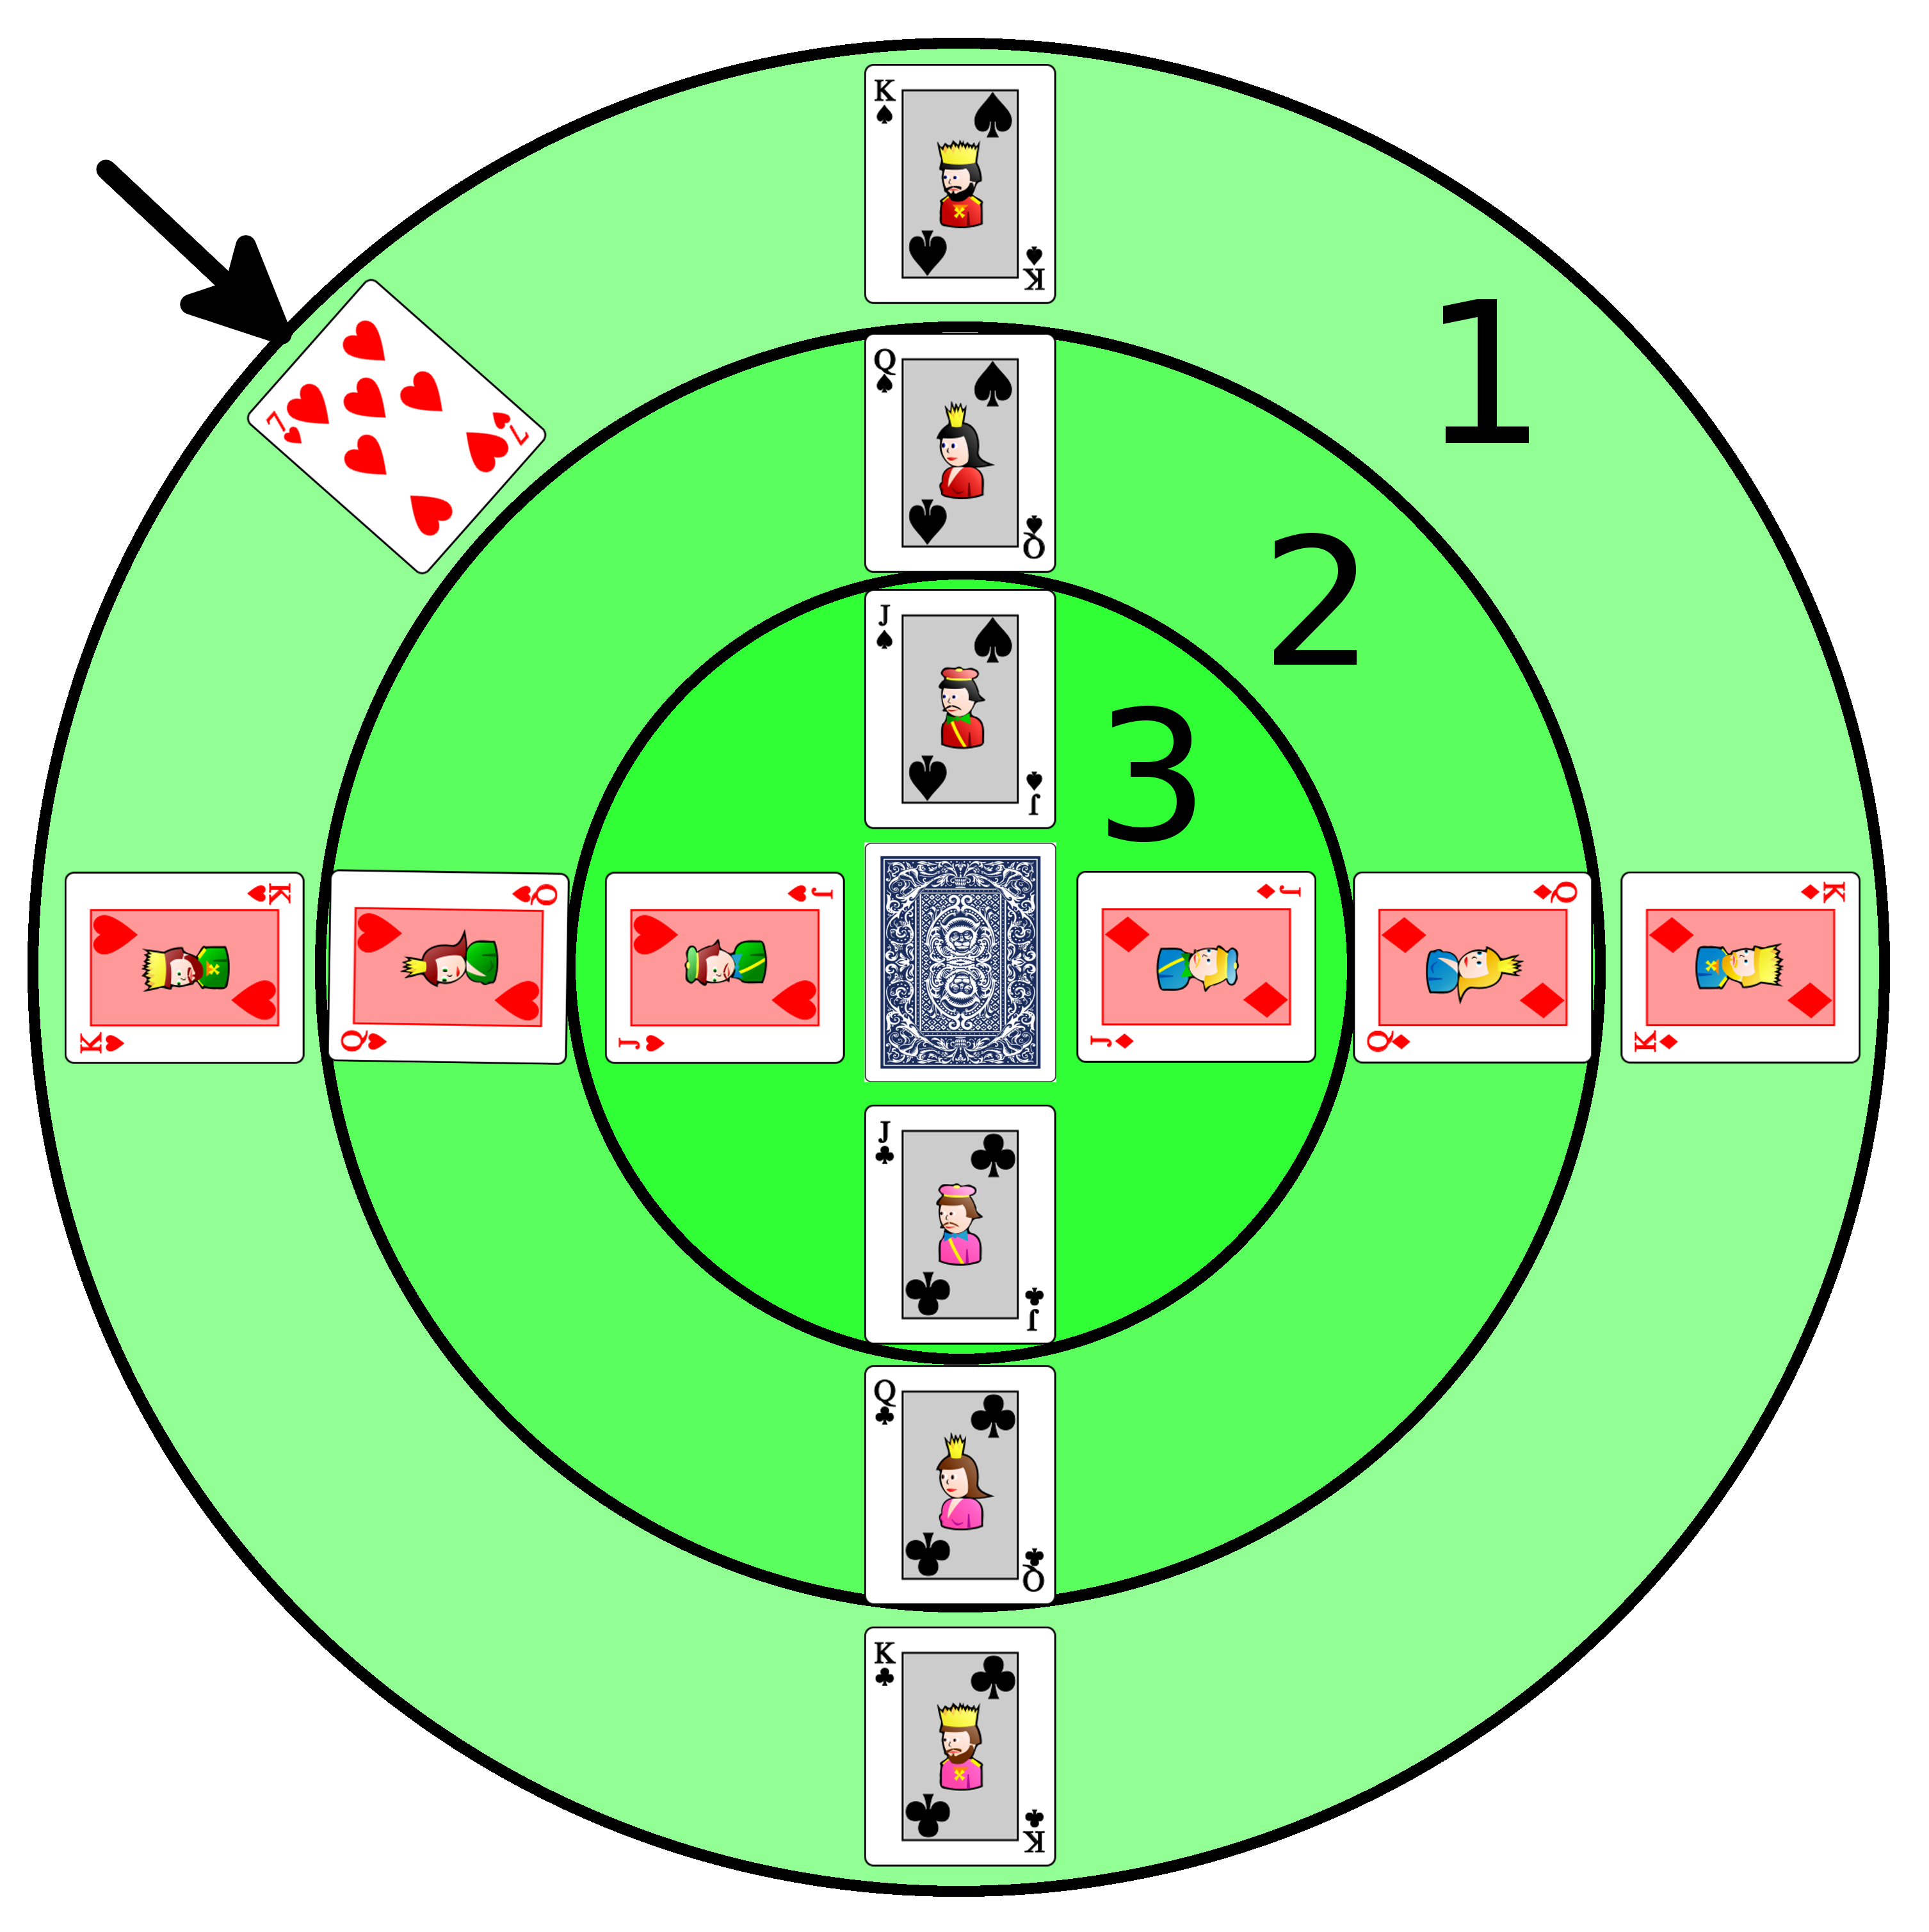
\includegraphics[scale=0.08]{draw.png}
\caption{Player Hearts draws 7 of Hearts and places it left of the Spire in which the King of Hearts resides}
\label{starting}
\end{figure}

\subsubsection{Attack-phase}
Each section of a Player's Spire (that is; his/her King, Queen and Jack) can attack one attacking Henchman per turn. However, the Henchman the Player wishes to attack must be in a corresponding \textit{Zone} in relation to the attacker Spire-Section. \\
E.g. if King of Hearts is at the top of a Spire, in \textit{Zone 1}, King of Hearts may attack any attacking Henchman in \textit{Zone 1}. \\
E.g. if Jack of Diamonds is in the middle of a Spire, in \textit{Zone 2}, Jack of Diamonds may attack any attacking Henchman in \textit{Zone 2}.\\

\noindent
Example (see Figure 3): \\
Player Hearts may attack card 7 of Hearts or 9 of Spades with King of Hearts. \\
Player Hearts may attack card 5 of Hearts, 2 of Diamonds or 4 of Clubs with Queen of Hearts. \\
If Progression-Rule 1 is used; the bottom cards will never have a chance to attack any Henchmen, and will only act as Shields. \\
If Progression-Rule 2 is used; the bottom cards can attack Henchmen in \textit{Zone 3}. \\

\noindent
Each Spire-Section may attack only once per turn. A player may choose not to attack anything if he/she so wishes.

\begin{figure}[h!]
\centering
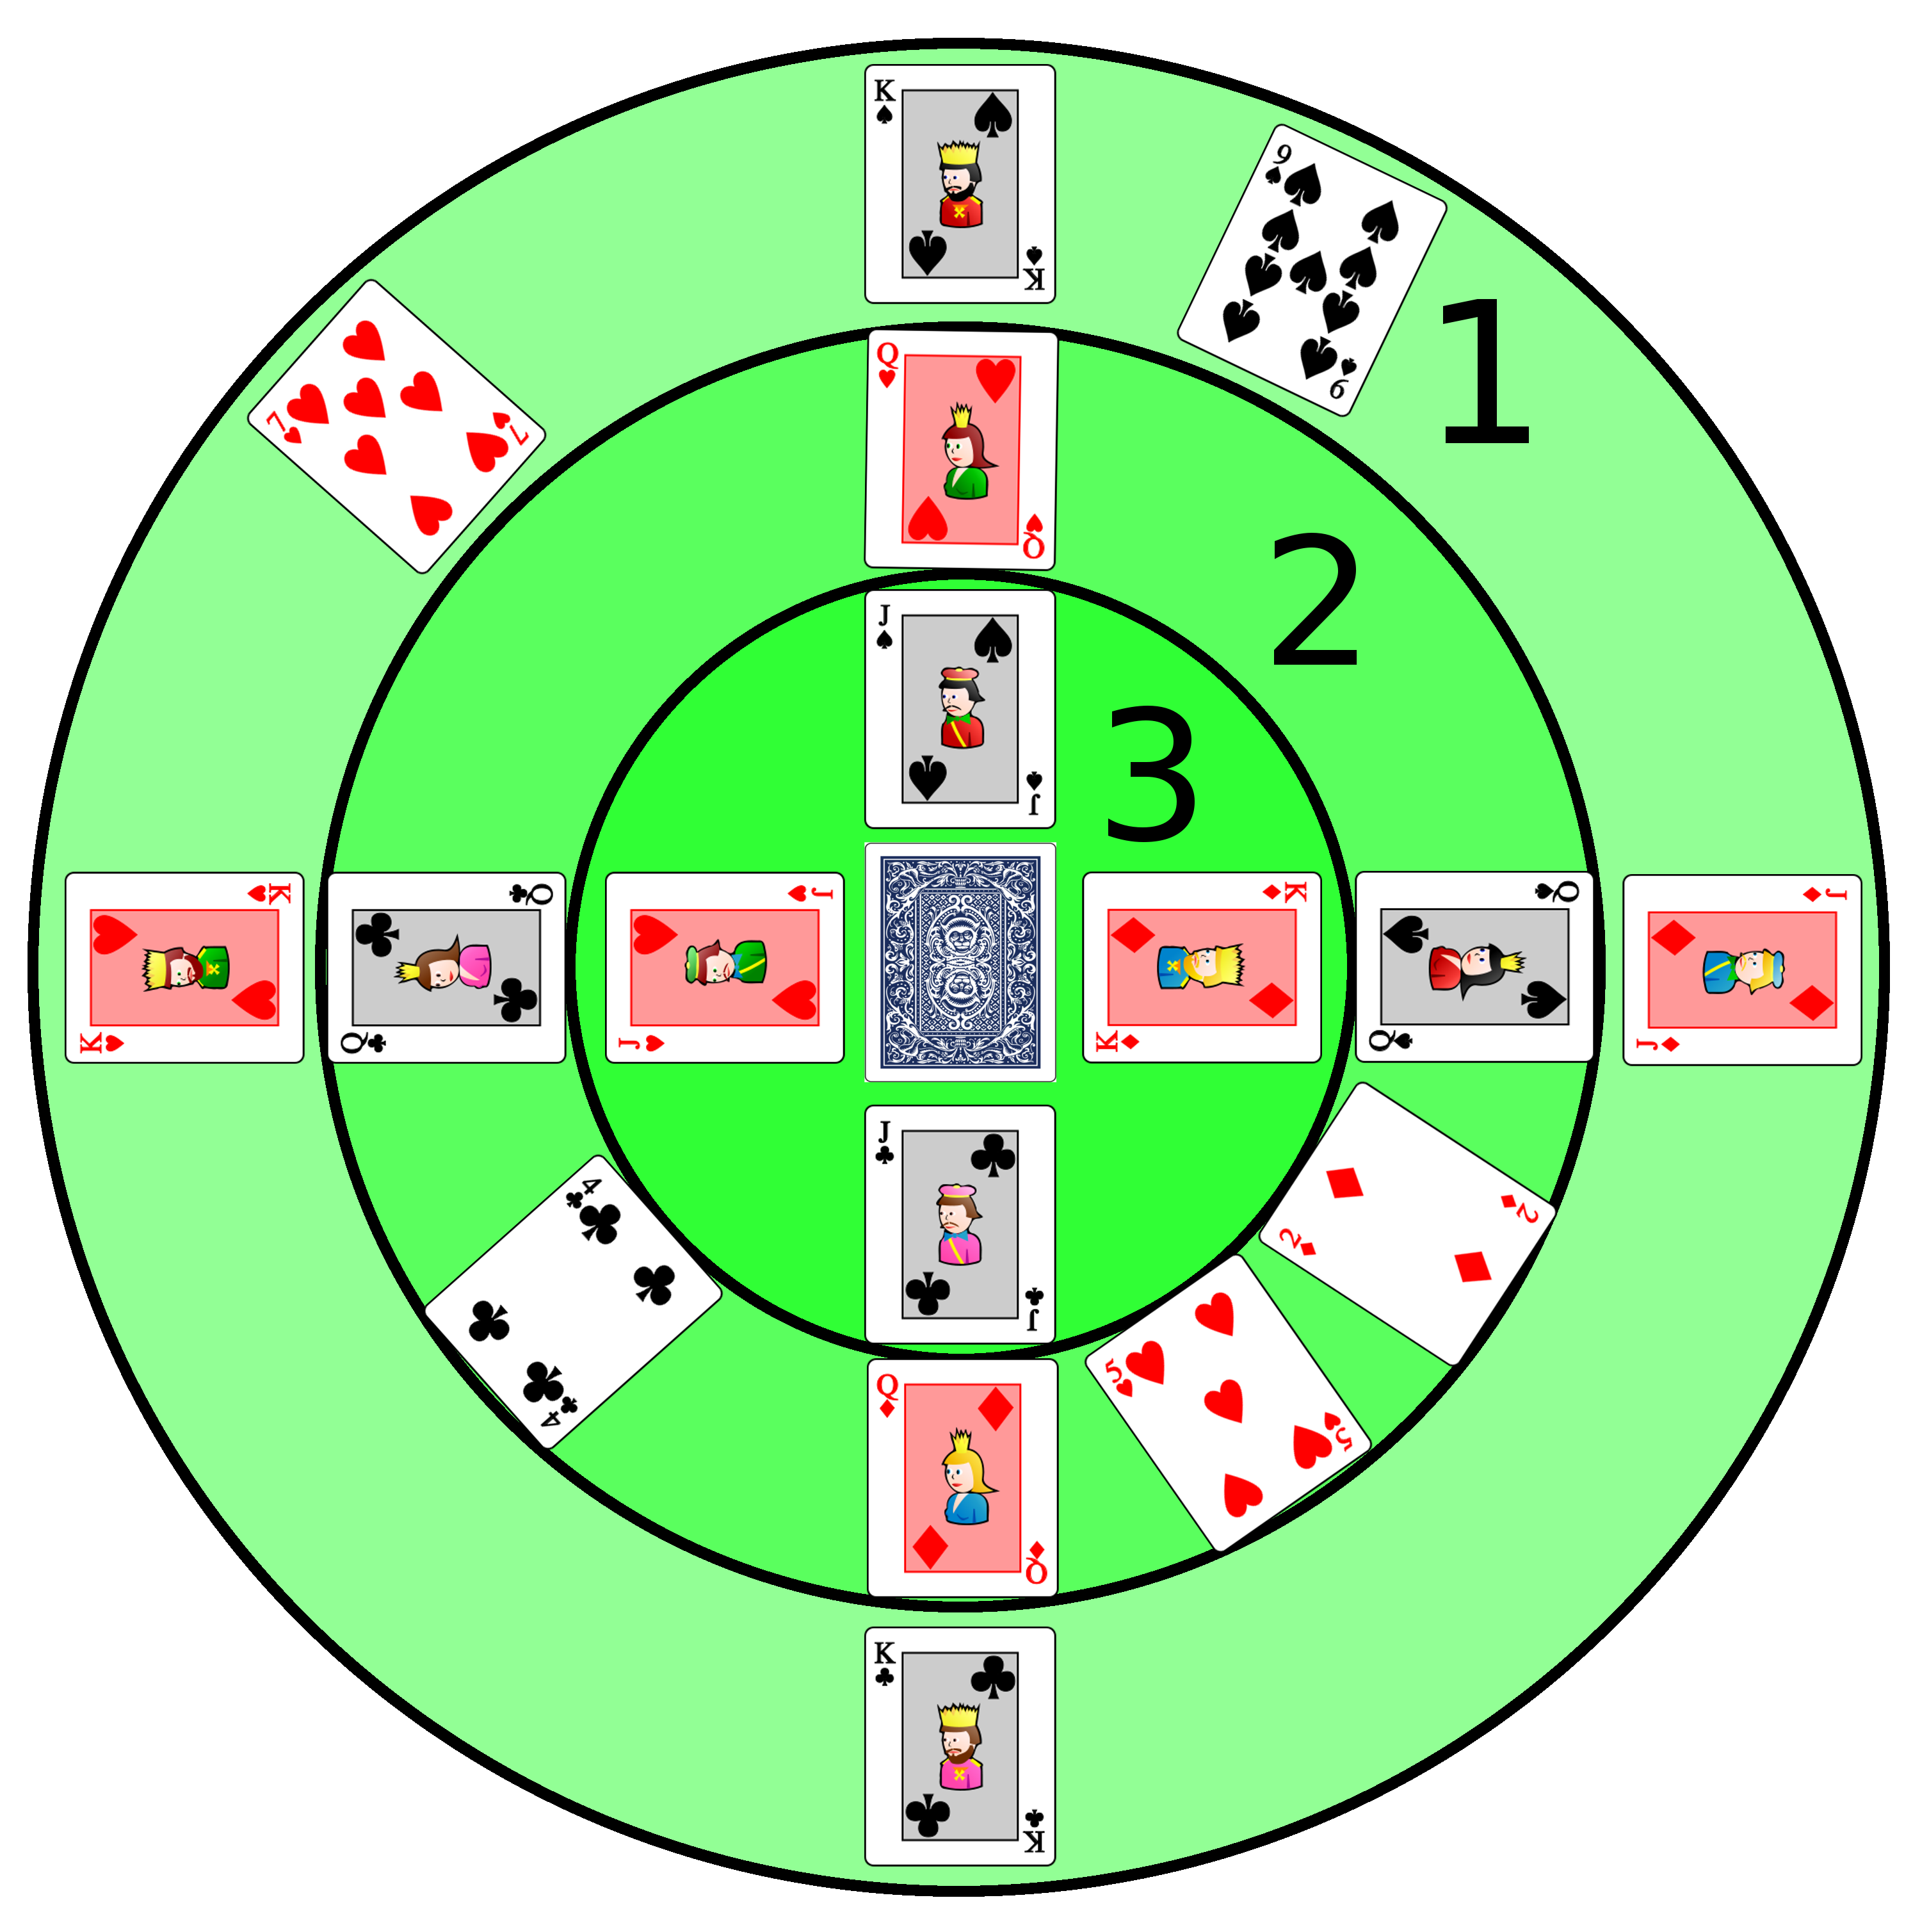
\includegraphics[scale=0.08]{attack.png}
\caption{A potential Attack-phase after a couple of turns}
\label{starting}
\end{figure}

\noindent
When a Player has chosen which Henchmen to attack - or which Henchmen not to attack - he/she will, for each attempted attack, roll the die to see whether or not the attack was sucessful. Since the Realm of Thin-Things spawns a great deal of very thin-things indeed, some of the Kings' Henchmen are very thin, and thin-things are hard to hit. \\
The Henchmen are numbered one through ten (two through ten, if you're playing with the Optional Rule described under Draw-phase) where smaller numbers describe thin-ness. \\
A player will have to roll either equal to-/or below the Henchmen's thin-ness in order to slay them. If a player has rolled above a certain Henchman's thin-ness the attack was un-sucessful and the Henchman stays on the board. \\
If the attack was sucessful, the Henchman is discarded.


\subsubsection{Shuffle-phase}
Each turn is ended with a roll on the \textit{Shuffle-Table} to decide how the Shuffling Spires shuffle during the Shuffle-phase. The \textit{Shuffle-Table} is described as follows: \\

\begin{tabular}{ l l }
1 & Bottom Section Right \\
2 & Bottom Section Left \\
3 & Middle Section Right \\
4 & Middle Section Left \\
5 & Top Section Right \\
6 & Top Section Left \\
7 & Shuffle Spire Downwards\\
8 & Shuffle Spire Upwards \\
9 &  Roll \textit{Shuffle-Table} twice\\
10 & - \\
\end{tabular}

\begin{figure}[h!]
\centering
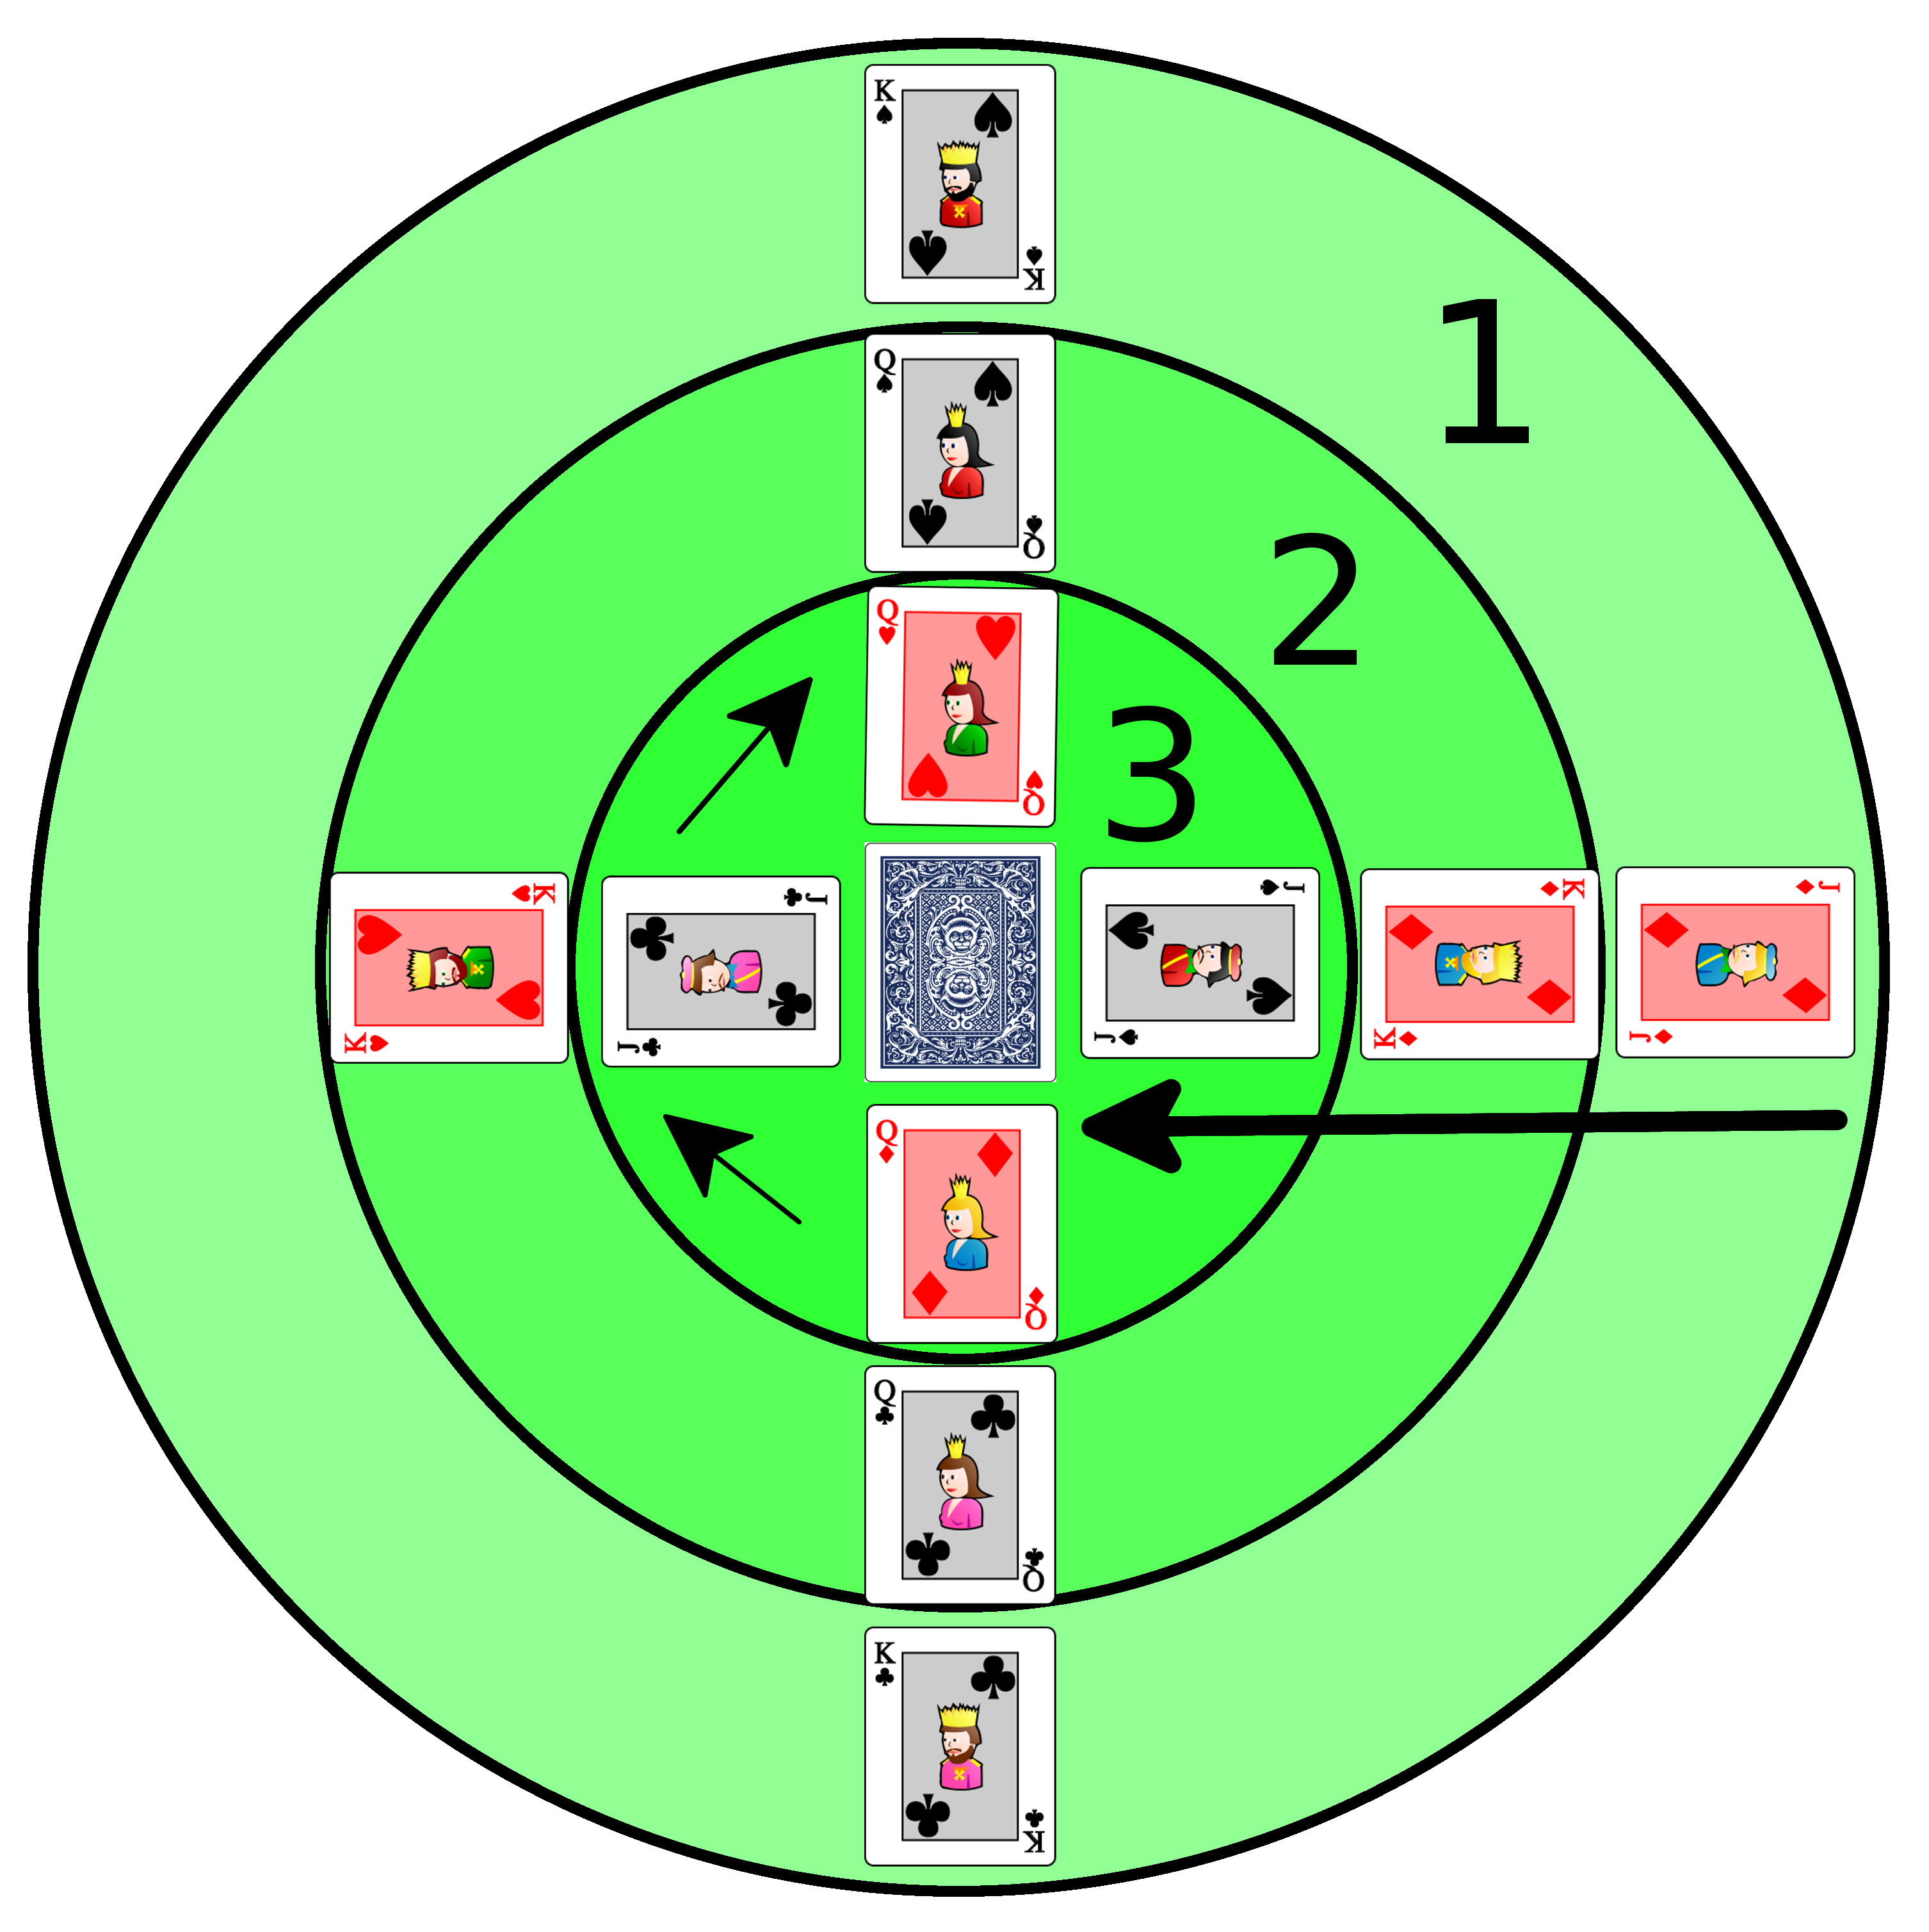
\includegraphics[scale=0.08]{shuffle.png}
\caption{Player Diamonds rolls a 9, followed by 7 and 2, on the \textit{Shuffle-Table}}
\label{starting}
\end{figure}

\subsubsection{Notes}
If another Spire-Section occupies your Shuffled Spire-Section's new position, then relocate that Spire-Section in accordance to the \textit{Shuffle} in question. \\
E.g. if all bottom \textit{Zones} on the board are occupied, and a player rolls 1 on the \textit{Shuffle-Table}, then move all bottom cards to the Right. \\

\noindent
If your newly moved Spire-Section isn't resting steadily on lower section, then lower it. These are very thin wind-swept Spires, not flying ones!

\subsection{Winning \textbf{Shuffle-Spires}}
\textbf{Shuffle-Spires} is a game about \textit{attempting} to predict the chaos the storm and winds have wrought upon the Kings of Thin, their Legendary Spires and their plan for Realm-Domination. \\
The objective in \textbf{Shuffle-Spires} is to be the sole surviving King of Thin (and thereof the ruler of the Realm of Thin-Things). \\
That is; to keep one’s top section (King) from being destroyed for as long as possible.

\subsection{Other}

\noindent
Playing Card models have been stolen from \href{''http://en.wikipedia.org/wiki/Playing_card#French_design''}{Wikipedia}. \\

\noindent
\textbf{Shuffle-Spires} was designed by \textit{me}, since - apparently - I have nothing better to do during summer than to develop card-games. I wish to thank my brothers and cousins for playtesting. \\
Enjoy! \\

\noindent
Eric Nilsson \\
CaterHatterPillar.com

\end{document}